\documentclass[11pt,letterpaper]{article}
\usepackage[lmargin=1in,rmargin=1in,bmargin=1in,tmargin=1in]{geometry}
\usepackage{../style}

\setlength{\parindent}{0ex}

% -------------------
% Content
% -------------------
\begin{document}

\pagenumbering{gobble}

% Recitation: Polynomials (Linear & Quadratic Functions)
\phantom{} \hfill {\bfseries \Large Recitation: Polynomials (Linear \& Quadratic Functions)} \hfill \phantom{} \par\vspace{0.5cm}

% Problem 1
\noindent {\bfseries Problem 1.} Sketch the function $f(x)= 7 - (x - 5)^2$.
	\[
	\fbox{
	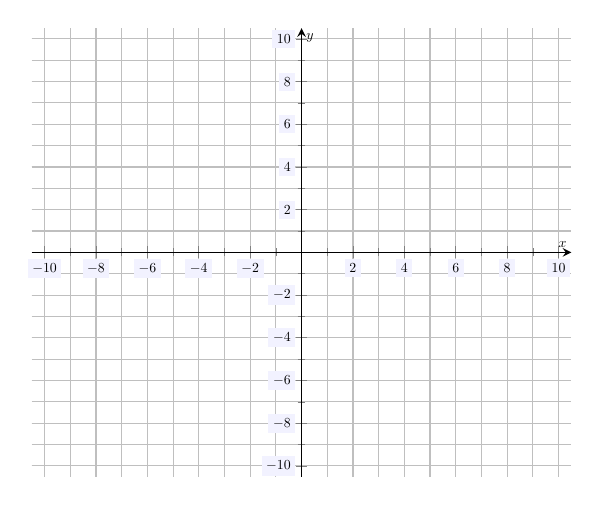
\begin{tikzpicture}[scale=1,every node/.style={scale=0.5}]
	\begin{axis}[
	grid=both,
	axis lines=middle,
	ticklabel style={fill=blue!5!white},
	xmin= -10.5, xmax=10.5,
	ymin= -10.5, ymax=10.5,
	xtick={-10,-8,-6,-4,-2,0,2,4,6,8,10},
	ytick={-10,-8,-6,-4,-2,0,2,4,6,8,10},
	minor tick = {-10,-9,...,10},
	xlabel=\(x\),ylabel=\(y\),
	]
	\end{axis}
	\end{tikzpicture}
	}
	\]



% Problem 2
\noindent {\bfseries Problem 2.} Find the equation of the quadratic function shown below. Be sure to fully justify why your answer is correct.
	\[
	\fbox{
	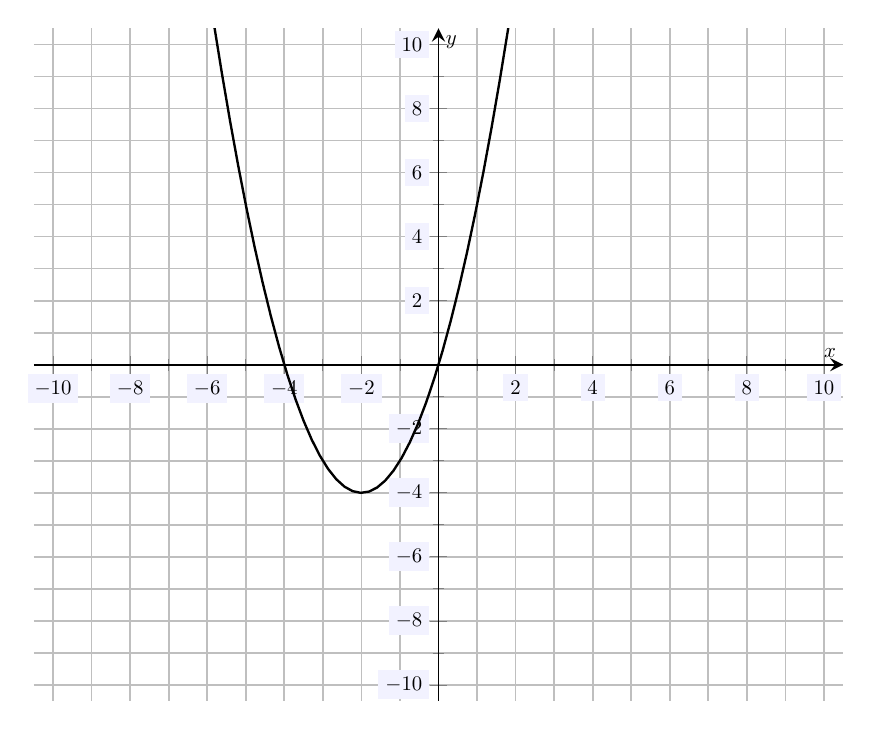
\begin{tikzpicture}[scale=1.5,every node/.style={scale=0.5}]
	\begin{axis}[
	grid=both,
	axis lines=middle,
	ticklabel style={fill=blue!5!white},
	xmin= -10.5, xmax=10.5,
	ymin= -10.5, ymax=10.5,
	xtick={-10,-8,-6,-4,-2,0,2,4,6,8,10},
	ytick={-10,-8,-6,-4,-2,0,2,4,6,8,10},
	minor tick = {-10,-9,...,10},
	xlabel=\(x\),ylabel=\(y\),
	]
	\addplot[line width= 0.02cm,samples=100,domain= -10.5:10.5] ({x},{(x + 2)^2 - 4});
	\end{axis}
	\end{tikzpicture}
	}
	\] 



\newpage



% Problem 3
\noindent {\bfseries Problem 3.} Solve the following equation:
	\[
	5\sqrt{2}\, x + 8= -3(1 - 2x)
	\] \vfill



% Problem 4
\noindent {\bfseries Problem 4.} Consider the quadratic function $f(x)= x^2 - 6x + 14$.
	\begin{enumerate}[(a)]
	\item Find $a, b, c$ for this quadratic function.
	\item Does $f(x)$ open upwards or downwards? Explain.
	\item Is this quadratic function convex or concave? Explain. 
	\item Find the minimum value of $f(x)$, if it exists. If it does not exist, explain why.  
	\item Find the maximum value of $f(x)$, if it exists. If it does not exist, explain why. 
	\end{enumerate} \vfill

\end{document}